\begin{figure*}[!tbp]
	\centering
        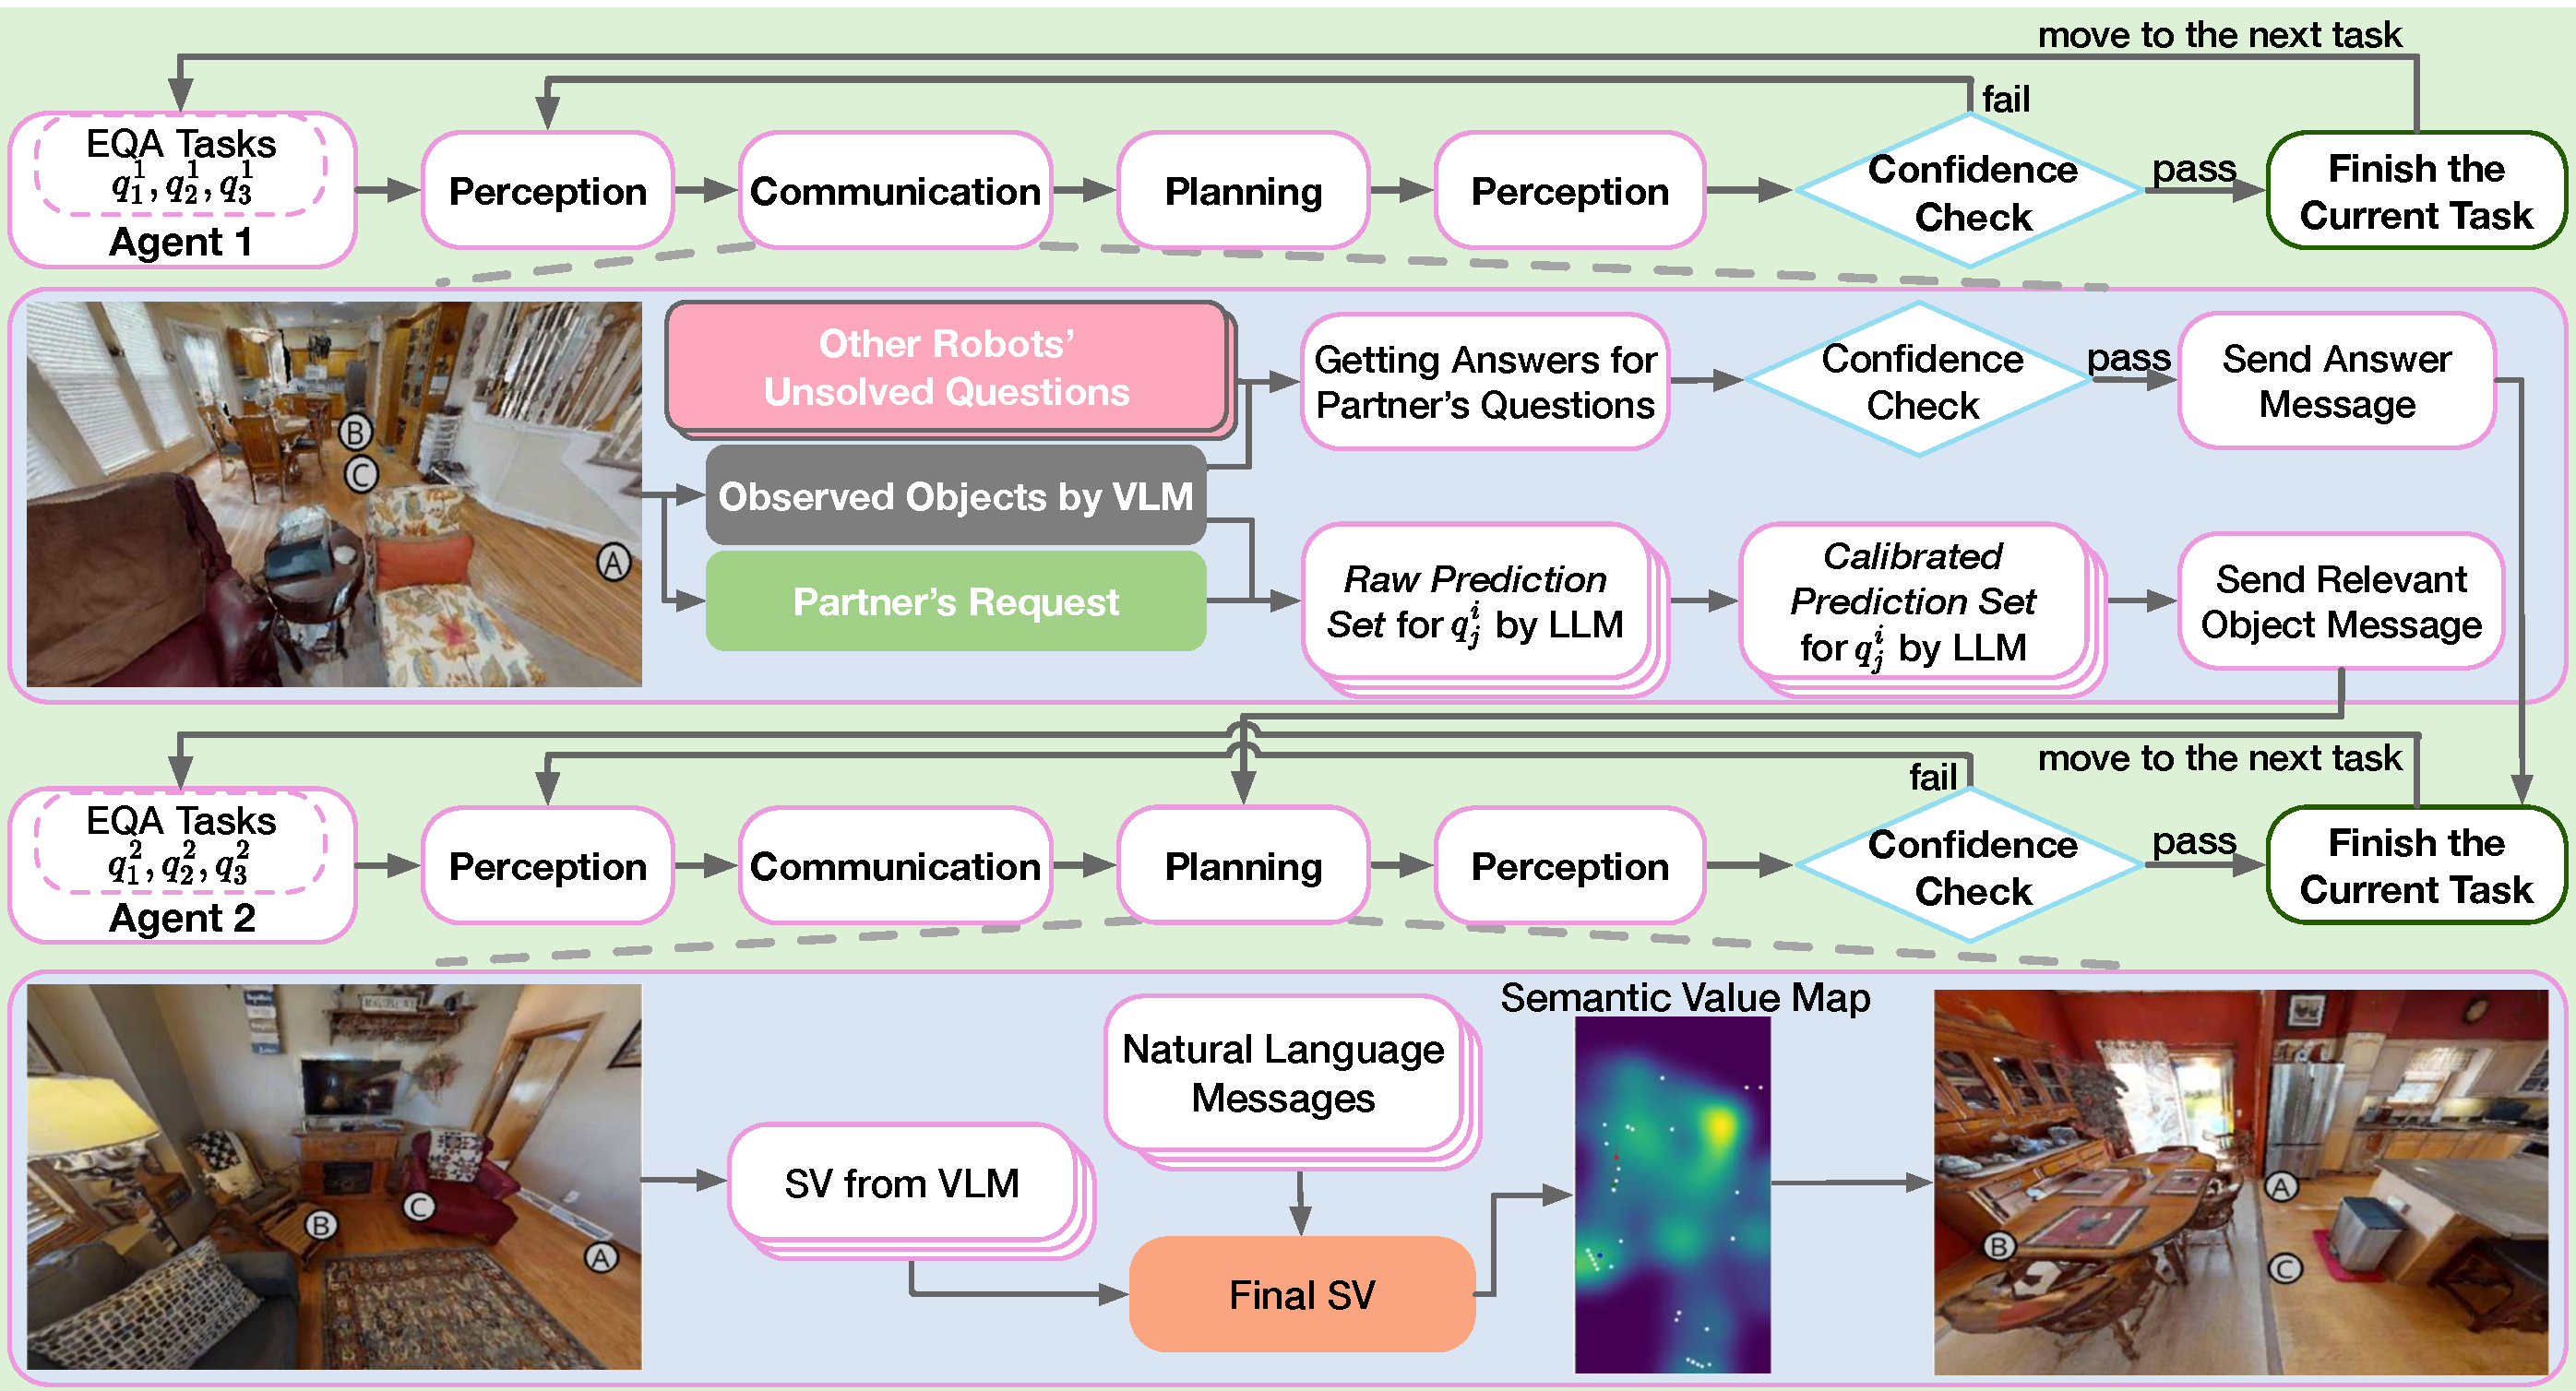
\includegraphics[width=\linewidth]{img/Fig2.pdf}
        \vspace{-0.5cm}
	\caption{An overview of our framework shows each robot with a perception module, a communication module, a planning module, and a confidence check module. At each time step, a robot generates local and global semantic values (SV) based on the current view and the communication message from the other robot. It navigates using a 2D weighted semantic value map and handles related object-check requests from other agents. The messages are generated based on the robot's current view, which are calibrated by conformal prediction to enhance relevance.}
    \vspace{-0.3cm}
    \label{fig:process}
\end{figure*}

This section introduces the CommCP framework, which leverages communication to enhance multi-agent exploration for the MM-EQA problem.
Building upon the approach presented in \cite{ren2024explore} for single-agent single-task EQA, our framework further enables communication capabilities to improve task completion efficiency and success rate. Furthermore, our framework can be easily extended to handle more complex human assignments in multi-agent settings, where robots are tasked with executing downstream tasks based on the information they acquire since robots are assigned questions based on their capabilities for the downstream tasks.


The overall framework architecture is illustrated in Fig.~\ref{fig:process}, which consists of four core modules: perception, communication, planning, and confidence check modules. The planning and confidence check modules are modified from \cite{ren2024explore}. In the communication module, messages are generated and projected onto the semantic value map in the planning module to guide the robots' exploration strategies. This module also enables a robot to provide answers to other robots' questions when it has sufficient confidence. All notations in this section correspond to time $t$.
For each robot $i$, the perception module employs a VLM to detect a set of observed objects $O^{i}_{\text{observe}}$ from the RGB image $I^i_{c}$ with the following prompt:

\vspace{+0.1 cm}
\colorbox{lime!20}{
\parbox{\dimexpr0.90\linewidth-2\fboxsep}{
\fontsize{8.5pt}{\baselineskip}\selectfont
\textit{
Consider the indoor scenario, analyze the provided image and list all the objects you observe. Provide the name of each object along with its color, separated by a comma. 
}
}}
\vspace{+0.1 cm}

The perception module's detected $O^{i}_{\text{observe}}$ are fed into the reasoning process to determine which objects to include in the communication by employing conformal prediction.
Each unsolved question is sequentially prompted to the LLM, along with 
$O^{i}_{\text{observe}}$, to generate an answer. 
If the answer passes the confidence check described in Sec. IV.D and the question is assigned to the responding robot, it proceeds. Otherwise, it sends the answer to the responsible robot. 
\subsection{LLM-Based Object Relevance Reasoning}\label{sec:A}
In indoor scenarios, objects are typically organized according to patterns of human usage, and LLMs can leverage the general knowledge of these patterns. 
Thus, if LLM assesses that an object observed in an area is highly relevant to the target object, there is an increased likelihood that the target is nearby. Based on this intuition, we design a communication framework that enables robots to share relevant object information or answers to other robots' questions.

During exploration, each robot $\hat{i}$ sends a request $r^{\hat{i}}_j$ to seek for assistance on its question $q^{\hat{i}}_j$ and provide its target objects $O^{\hat{i}}_{\text{request}}$. 
The LLM evaluates objects observed by robot $i$, denoted as $O^{i}_{\text{observe}}$, and the observed and target objects are labeled as \textbf{Observed} and \textbf{Request}, respectively. We employ the zero-shot chain-of-thought \cite{kojima2022large} to prompt the LLM to conduct detailed reasoning before generating a final output. 
The following is the prompts used for the LLM. Here, the \textit{system prompt} is the instruction for the LLM, and the \textit{user prompt} is the content of the conversation with LLM.

\vspace{+0.1 cm}
\colorbox{lime!20}{
\parbox{\dimexpr0.90\linewidth-2\fboxsep}{
\raggedright
\fontsize{8.5pt}{\baselineskip}\selectfont
\textbf{System prompt:} \\
\textit{As a robot in a house, your partner is looking for \{\textbf{Request}\} and you can inform them about what you have observed.}
}}


\colorbox{lime!20}{
\parbox{\dimexpr0.90\linewidth-2\fboxsep}{
\fontsize{8.5pt}{\baselineskip}\selectfont
\textbf{User prompt:} \\
\textit{You observe \{\textbf{Observed}\}. Your partner wants to find \{\textbf{Request}\}. Since you and your partner are not in different locations, evaluate whether it is worth it for your partner to travel to your position to find \{\textbf{Request}\}.\\ 
You have four options: \textbf{A} (Yes. Because \{\textbf{Request}\} and \{\textbf{Observed}\} are same, 
and you might directly find \{\textbf{Request}\}).}
\textit{
\textbf{B} (Yes. They are highly relevant. This means \{\textbf{Request}\} should be close to \{\textbf{Observed}\}).
\textbf{C} (No. They are not strongly related).   
\textbf{D} (No. \{\textbf{Observed}\} is a common feature).}

\textit{For option A, consider if \{\textbf{Observed}\} and \{\textbf{Request}\} are the same things.  
For option B, consider where \{\textbf{Request}\} is most likely to be found. Then evaluate if \{\textbf{Observed}\} is likely to appear in that location as well. 
For options C and D, since you and your partner are not in the same position, assess if \{\textbf{Observed}\} is worth passing by. 
Option D implies that \{\textbf{Observed}\} is just a common feature in the house. 
Now provide your analysis.}
}}
\vspace{+0.13 cm}

The LLM's output, \textit{\textbf{Analysis}}, is used to compute probabilities for each option. We employ the following prompt that directs the LLM to select only one option based on \textit{\textbf{Analysis}}.

\vspace{0.13cm}
\colorbox{lime!20}{
\parbox{\dimexpr0.90\linewidth-2\fboxsep}{
\fontsize{8.5pt}{\baselineskip}\selectfont
\textbf{System prompt:} \\
\textit{You should only output one letter.} \\
\textbf{User prompt:} \\
\textit{
Your observe $O^{\text{observe},i}_{t,k}$ now. Your partner wants to find \{\textbf{Request}\}. 
Since you are in different locations, you need to assess if it's worthwhile for your partner to come for \{\textbf{Request}\}. 
You have four options: \textbf{A, B, C, D}. Here is your previous analysis: \{\textbf{Analysis}\}. You should only output one letter.}
}}
\vspace{0.13cm}

Each observed object for robot $i$ is assigned an \textit{option-probability pair} $O^{i}_{\text{observe},k} := \{\text{Option}_k, p_k \mid k=1,...,N_{k}\}$, where $N_k$ is the number of observed objects and $p_k$ is the probability of the token corresponding to $\text{Option}_k$ generated by the LLM. 
If  \textbf{Option A} is returned, it is likely to correspond to the target object $O^{i}_{\text{target},j}$ of request $r^{\hat{i}}_j$. 
If \textbf{Option B} is selected, it is likely a relevant object $O^{i}_{\text{relevant},j}$ related to request $r^{\hat{i}}_j$. 
Objects with options C and D are disregarded.

\subsection{Message Generation with Conformal Prediction}

To mitigate potential miscalibration in LLM-generated lists of targets and relevant objects, which leads to irrelevant information, we employ conformal prediction (CP) \cite{shafer2008tutorial} to calibrate object lists for message generation. 
CP provides statistically guaranteed prediction sets that contain the ground truth with a user-specified probability \cite{ren2023robots}.
Specifically, we adopt split conformal prediction \cite{fontana2023conformal}, which involves designing a conformity score to measure the reliability of predictions, collecting a calibration set to establish standards for comparing conformity scores during testing, and determining whether to include a prediction result in the final prediction set. 
In the context of deep learning, the conformity score is defined as the probability output of models as this reflects its confidence in the answers it produces.

In our framework, we adopt $p_k$ as conformity scores, and only $\text{Option}_k$ with $p_k$ higher than a computed threshold are included in the calibrated prediction set. To handle different probability distributions for \textbf{Options A} and \textbf{Options B}, we define two calibration sets: \( \mathcal{Z}^{A}_{\text{cal}} = \{ z_k = (\text{`A'}, p_k) \mid k=1,..., N_k\} \) and \( \mathcal{Z}^{B}_{\text{cal}} = \{ z_k = (\text{`B'}, p_k) \mid k=1,..., N_k\} \). 
To collect the calibration sets, we sample (observed\_object, target\_object) pairs from 20 diverse HM3D scenarios and generate ground truth labels. To handle scenarios where multiple objects may be relevant, we formally define the ground truth for calibration as the single option with the highest LLM confidence score, following the procedure in \cite{ren2023robots}. For each labeled pair, we apply the LLM reasoning process described in Section V.A to obtain probability values $p_A$ and $p_B$, which form the calibration sets $\mathcal{Z}^{A}_{\text{cal}}$ and $\mathcal{Z}^{B}_{\text{cal}}$, respectively. 
These calibration datasets represent samples from the underlying distributions $\mathcal{D}^{A}_{\text{cal}}$ and $\mathcal{D}^{B}_{\text{cal}}$ for spatial co-occurrence judgments in household environments. 
Let $\mathcal{D}^{A}_{\text{test}}$ and $\mathcal{D}^{B}_{\text{test}}$ represent the unknown distributions of option-probability pairs for a new scenario, which are assumed to be exchangeable with $\mathcal{D}^{A}_{\text{cal}}$ and $\mathcal{D}^{B}_{\text{cal}}$.


In our MM-EQA setting, we argue that calibration and test samples can be treated as independent and identically distributed (i.i.d). Let $(s_i, p_i)$ represent the $i$-th sample, where $s_i$ denotes the spatial relationship (A or B) and $p_i$ denotes the LLM's probability output. Our i.i.d. assumption states:
\vspace{-0.15cm}
\begin{equation}
P((s_1, p_1), (s_2, p_2), \ldots, (s_n, p_n)) = \prod_{i=1}^{n} P(s_i, p_i),
\vspace{-0.15cm}
\end{equation}
where $(s_i, p_i) \sim F$ for all $i$, and $F$ is a fixed joint distribution over spatial relationships and probability values. 
This assumption holds because the calibration process satisfies both independence and identical distribution requirements: 
1) Calibration scenarios are randomly sampled from the HM3D household dataset without temporal or spatial dependencies; 
2) Each (observed\_object, target\_object) evaluation represents an independent semantic judgment; 
3) LLM's probability outputs for different object pairs are not causally related; 
4) Spatial co-occurrence patterns represent typical household organization principles; 
5) The LLM's semantic understanding remains consistent across scenes; 
6) The underlying distribution $F$ of object spatial relationships is preserved across the dataset; 
and 7) During testing, each robot generates semantic values for target and relevant objects based solely on its current view, without considering past frames, which ensures spatial and temporal independence required for conformal prediction.
Fulfilling these conditions ensures that the prerequisite for applying conformal prediction is met.
While CP typically requires only exchangeability of data, our i.i.d. assumption provides stronger theoretical guarantees. 
Approximately $1/\delta$ calibration samples are needed for reliable coverage~\cite{luo2024sample}, and 20 scenarios provide adequate data to achieve typical confidence levels (e.g., $\delta = 0.05$).

For a new test sample \( z_{\text{test}} = (\text{`A' or `B'}, p_{\text{test}}) \), we use CP to construct a prediction set $\mathcal{C}(z_{\text{test}})$ using a calibrated score threshold, $p_{\text{thres}}$. 
This threshold is set to the $1-\epsilon_1$ quantile of the scores in the calibration set, where \( \epsilon_1 \) is a user-defined miscoverage rate (e.g., $\epsilon_1=0.05$ for 95\% confidence) that influences the size of the prediction set \( \mathcal{C}(\cdot) \). 
The prediction set is then formed by including all options whose scores, $p_{\text{test}}$, meet or exceed this threshold. 
This construction provides the formal marginal guarantee that the true label is contained within the prediction set with high probability:
\vspace{-0.15cm}
\begin{equation}
    P(z_{\text{test}} \in \mathcal{C}(z_{\text{test}})) \geq p_{\text{thres}}
    \vspace{-0.15cm}
\end{equation}
A higher $p_{\text{thres}}$ leads to more confident options being shared during communications, and vice versa.
The corresponding $O^{i
}_{\text{relevant},j}$ and $O^{i}_{\text{target},j}$ of the correct options along with approximate positions of correct options are used to generate the message \( \zeta^{i} \) using the template: ``I see \{relevant object\} that may be relevant to
your target \{true target\}, and \{possible target object\} may be your target at \{position\}.'' If neither object is identified, the robot will not send a message.

\subsection{Exploration with Communication}\label{sec:baseline_method}

To guide exploration, we first compute the semantic values (SV) $\text{SV}^i_{\text{no-com},j}$ for a 2D grid map as per \cite{ren2024explore}, ignoring the messages received from other agents. 
We denote $P$ as a set of frontier points identified by the VLM at the current pose— locations on the boundary of the explored and unexplored regions \cite{yamauchi1997frontier}.
The SV of ${\hat{p}} \in P$ is denoted as $\text{SV}^i_{{\hat{p}},j}$. 
Upon receiving a message \( \zeta^{\hat{i
}} \),  the SV for each ${\hat{p}} \in P$ based on communication is adjusted based on the counts of the relevant and target objects, scaled by temperature \( \tau_{1} \) and \( \tau_{2} \):
\vspace{-0.15cm}
\begin{equation}
\text{SV}^i_{\text{com},{\hat{p}},j} = \log\left(\tau_{1} \text{Num}(O^i_{\text{relevant},j}) + \tau_{2} \text{Num}(O^i_{\text{target},j})\right),
\end{equation}
where $\tau_1$ and $\tau_2$ weight the counts of relevant and target objects, respectively, balancing indirect semantic cues and direct task information in the communicated semantic value. For each task, the SV is defined as:
\vspace{-0.15cm}
\begin{equation}
\text{SV}^i_{{\hat{p}},j}= \max(\text{SV}^i_{\text{no-com},{\hat{p}},j}, \text{SV}^i_{\text{com},{\hat{p}},j})
\vspace{-0.15cm}
\end{equation}
The semantic value at position $\hat{p}$ is set to the maximum of the agent’s own estimate and the value from received messages, favoring the most informative source. The average of all $\text{SV}^i_{j}$ values is computed to determine the final semantic value:
\vspace{-0.15cm}
\begin{equation}
\text{SV}^i_{\text{final},{\hat{p}}} = 
\frac{1}{N_q} \sum_{j=1}^{N_q} \text{SV}^i_{{\hat{p}},j}
\vspace{-0.15cm}
\end{equation}

If $\text{SV}^i_{\text{final},{\hat{p}}}=0$, the robot randomly selects one of the frontier points to continue exploration. After moving, the robot applies Volumetric Truncated Signed Distance Function (TSDF) Fusion \cite{newcombe2011kinectfusion, zeng20173dmatch} to update the occupancy of the voxels in $M$, which marks them as explored or unexplored based on depth images $I^i_{d}$. This data is projected onto a 2D grid map matching the size of SV maps. The robot then uses Frontier-Based Exploration (FBE) \cite{yamauchi1997frontier} for path planning, where higher SV points indicate the surrounding areas likely to be more informative.
To improve exploration efficiency, Gaussian smoothing spreads each SV point's value across its surrounding region, enabling smoother navigation and helping robots prioritize areas with high information value.

\subsection{Confidence Check}

The robot performs a confidence check to determine if it has sufficient certainty to answer an embodied question. Here, we prompt the VLM to generate answer prediction probabilities over the four possible answers from $\{\text{`A', `B', `C', `D'}\}$, along with a question-image relevance score.  This relevance score reflects the likelihood that the robot’s current view contains the information needed to answer the question.
The VLM's probability of predicting ``Yes" to the prompt ``Consider the {question}. Are you confident about answering the question given the current view?" is regarded as the question-image relevance score 
$\text{Rel}^i_{j}$ for question $q^i_j$.
The set of answer probabilities is defined as $\{\text{Ans}^i_{j}(L) \mid \ L \in \{\text{`A', `B', `C', `D'}\}\}$.
Both $\text{Rel}^i_{j}$ and $\text{Ans}^i_{j}(L)$ are bounded within the interval $[0,1]$. The answer is considered confident, and subsequent exploration will exclude question $q^i_j$, if the following condition is met:
\(
\exists ! L \in \{\text{`A', `B', `C', `D'}\} \ \text{s.t.} \ \text{Ans}^i_{j}(L) \times \text{Rel}^i_{j} > 1 - \epsilon_2,
\)
where \( \epsilon_2 \) is a user-defined threshold that reflects the confidence level needed for termination. This threshold \( \epsilon_2 \) is applied to all robots when determining if an answer can be accepted.

\subsection{Stop Criterion}
In our setup, the robot terminates its exploration once it has answered all the questions assigned to it, either through its own analysis based on its observations and reasoning or with answers provided by the other robots. Alternatively, exploration stops when the maximum allowed time is reached.

\begin{figure*}[!tbp]
    \centering
    
\includegraphics[width=\linewidth]{img/Fig3.pdf}
    \vspace{-0.7cm}
    \caption{The diagrams of SC vs. NTC on our MM-EQA dataset.  (a)–(d) show the results for a 2-robot team. 
    (a) The comparison between our method and baselines. 
    (b) The ablative comparison of communication and conformal prediction modules.
    (c) The ablative comparison of the number of objects in the communication messages and the answering sharing mechanism. 
    (d) The ablative comparison of baselines with our method at message-sending speeds of 0.25, 0.5, 1, 2, and 4 messages per second.  
    (e) A scalability analysis comparing our method and baselines using a 3-robot team.}
    \vspace{-0.6cm}
    \label{fig:result_include1}
\end{figure*}
